\documentclass[a4paper, 12pt]{report}
\usepackage{graphicx}
\usepackage{float}
\usepackage{fixltx2e}
\usepackage{rotating}

\begin{document}
\begin{titlepage}
\begin{center}

\LARGE{Electronics and Computer Science}\\
\LARGE{Department of Physical and Applied Sciences}\\
\LARGE{University of Southampton}\\
\vfill
\normalsize{Thomas Scarsbrook}
\vfill
\normalsize\today

\vfill

\normalsize{Supervisor: Steve Gunn}\\
\normalsize{Examiner: Rob Maunder}

\vfill

\large{A project progress report submitted for the award of\\
MEng Electronic Engineering with Mobile and Secure Systems}

\end{center}
\end{titlepage}


\abstract{There are many undesired sounds around us all the time.
These sounds can often be very distracting to what we are attempting to hear.
There are various methods we can employ in an attempt to reduce the effect of these undesired sounds
So far I have experimented with one method of cancelling these out with a measured amount of success, however it is not optimal and suffers from some physical limitations.
I am also looking into an alternative, potentially much faster method of achieving the cancellation.
}
\addcontentsline{toc}{section}{Abstract}
\setcounter{page}{2}

\tableofcontents
\addcontentsline{toc}{section}{Contents}

\listoffigures
\addcontentsline{toc}{section}{List of Figures}

\listoftables
\addcontentsline{toc}{section}{List of Tables}

\chapter*{Acknowledgements}
I would like to thank my supervisor Steve Gunn for all his support and advice
during this project.
I would also like to thank the members of Student Robotics, who not only helped
me come up with the idea of this project, but also introduced me to many of the
pieces of software used in the project.
Also there are all the people who assisted with the proof reading of the
reports, including a couple of the people on my course, my parents, and some of
my sixth form teachers.

\addcontentsline{toc}{section}{Acknowledgements}

This is text \cite{EMHeadsets}
This is other text \cite{EMNoiseCancel}

This is more \cite{ICAAlg&Apps} text\\
Then you get some text about psychoacoustics \cite{MusCogCompSou} and about the DELAYS in sound waves, and how the ear uses them.

WOW, THIS SOURCE\cite{AdvancedDSPing} IS FANTSATIC, Shame that it seems innaccesable without spending \textsterling50\ldots \\
I especially reccommend looking at Page 12, it contains a great diagram!

\chapter{Introduction}

\chapter{Background}

\chapter{Planning}

\chapter{Modelling}
\section{Matlab}
In order to aid the design of the algorithms matlab models were produced and
tested.


\section{Hardware}
Much of the hardware used in this project is not possible to simulate, due to
the nature of the integrated circuits involved.
However, one aspect that can be simulated is the analogue circuitry before the
codec.

\subsection{Signal Conditioning}
Models of the signal conditioning were created in OrCAD in order to check that
the break frequency and roll off were suitable.
The design of this circuitry will be discussed later, in section
\ref{sec:imple:hard:sch} - only the modelling of it will be covered here.
The result of this modelling can be seen in figure \ref{fig:sigcondmodel}.
\\
\\
This graph shows that the signal conditioning amplifier has a break frequency
of 19409Hz.
This is ideal for the function it will be providing, as it is just below the
boundary of human hearing, meaning that all audible frequencies will reach 
the codec for sampling, while frequencies that would produce aliasing are
nullified.

\begin{figure}[H]
	\centering
	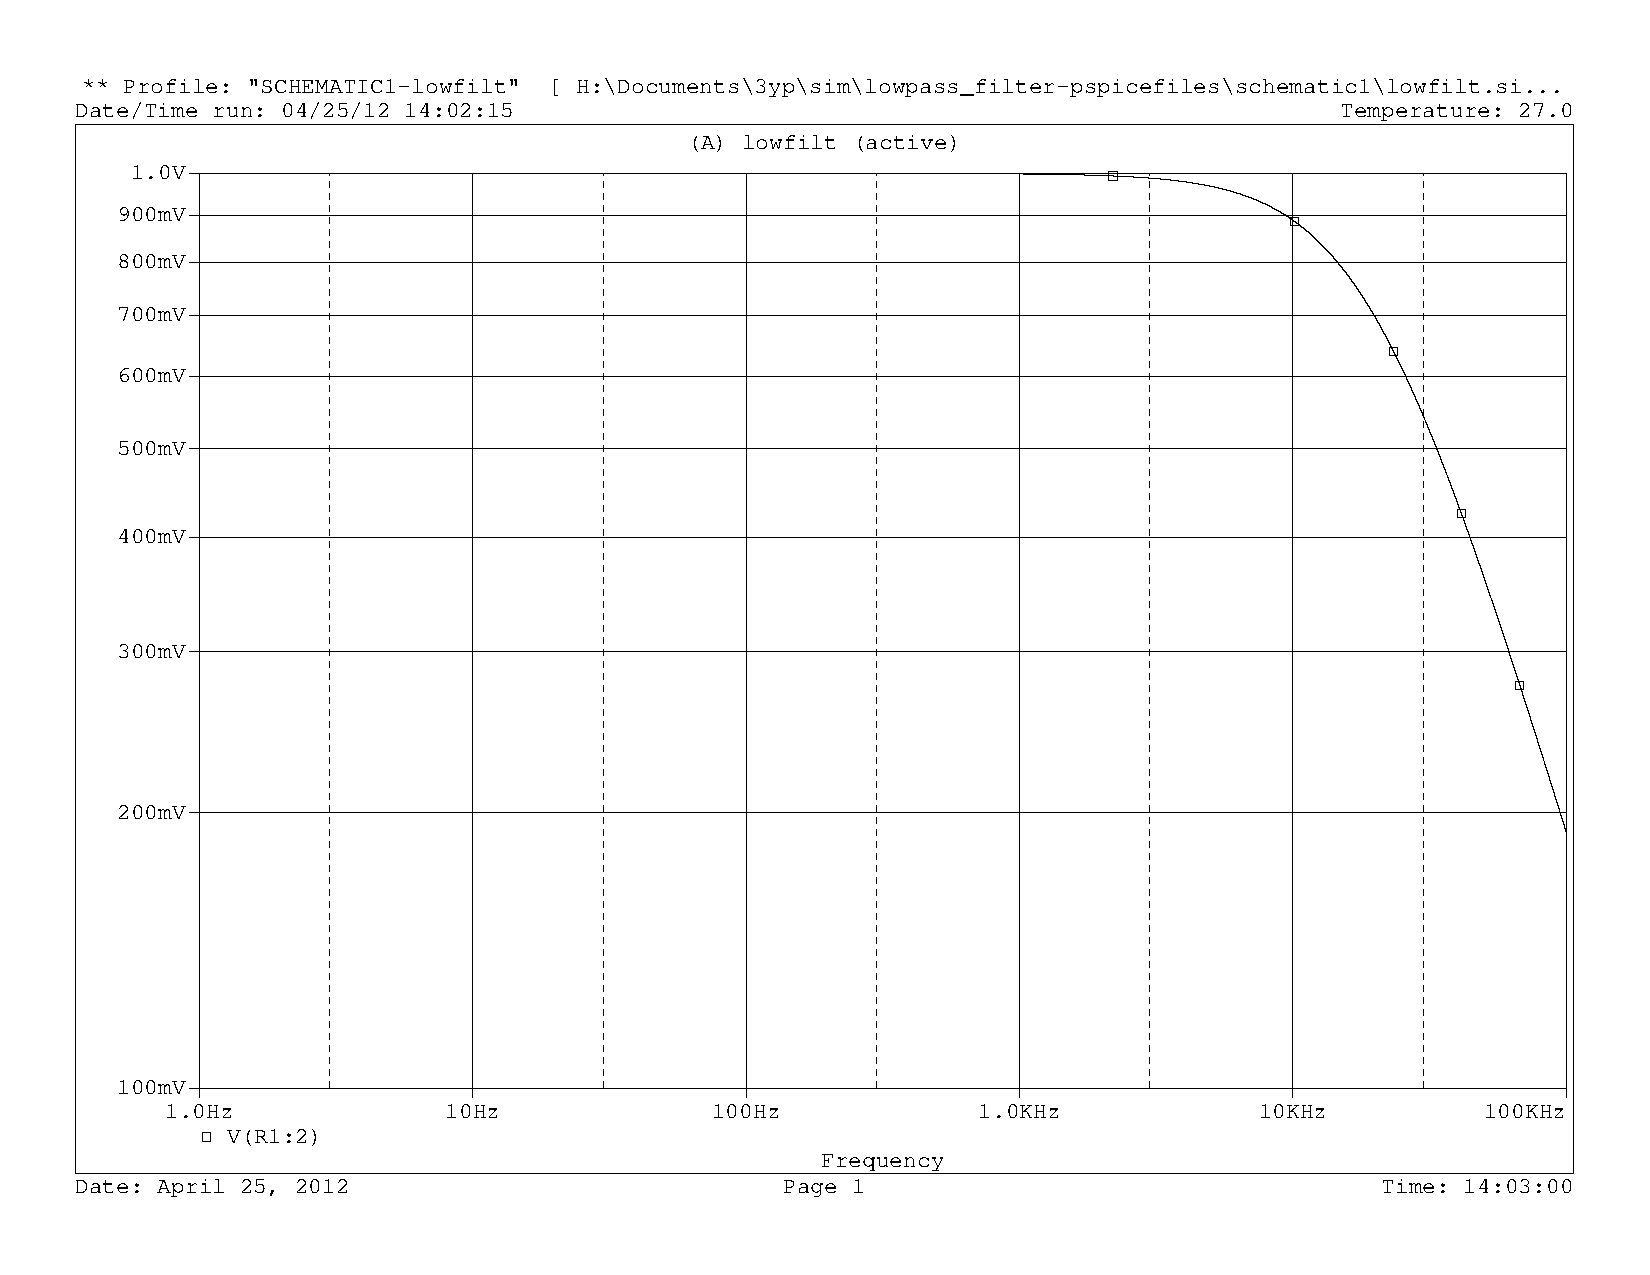
\includegraphics[width=\textwidth]{./img/signal_conditioning_sim.pdf}
	\caption{Simulation results of the signal conditioner}
	\label{fig:sigcondmodel}
\end{figure}

\subsection{Summing Amplifier}
A model of the summing (or instrumentation) amplifier was produced to check that it would function
as desired.
As the amplifier being used was not originally conceived for the use to which
it is put to in this project, modelling was even more important to check that
it would function as desired.
Although the produced amplifier would operate on two channels, as these channels
are identical, only one was simulated.

\begin{figure}[H]
	\centering
	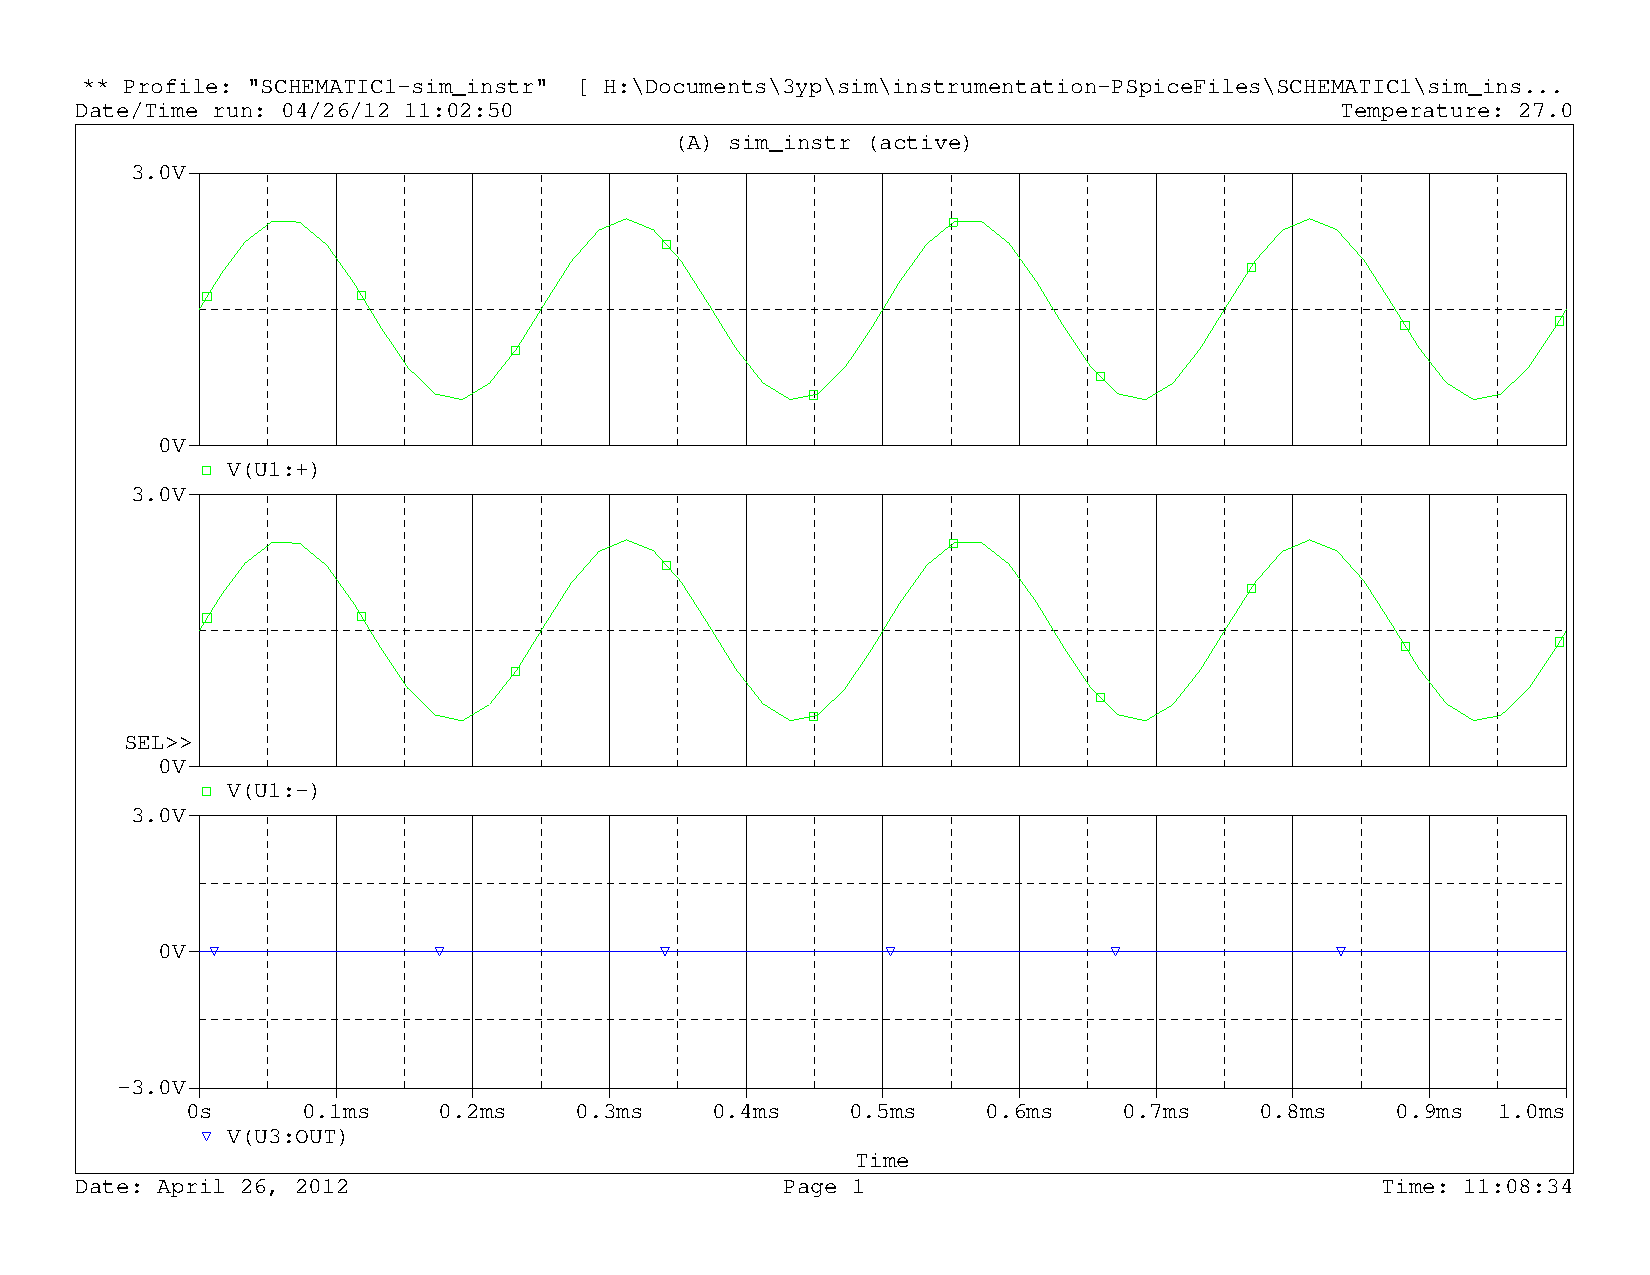
\includegraphics[width=\textwidth]{./img/instrumentationamp.pdf}
	\caption{The output from the instrumentation amplifier from two identical sine waves}
	\label{fig:instramp}
\end{figure}

\noindent Figures \ref{fig:instramp} and \ref{fig;instrampbeat} show that the summing amplifier will correctly sum the two signals together, with one of the signals experiencing a 180$^{\circ}$ phase shift.

\begin{figure}[H]
	\centering
	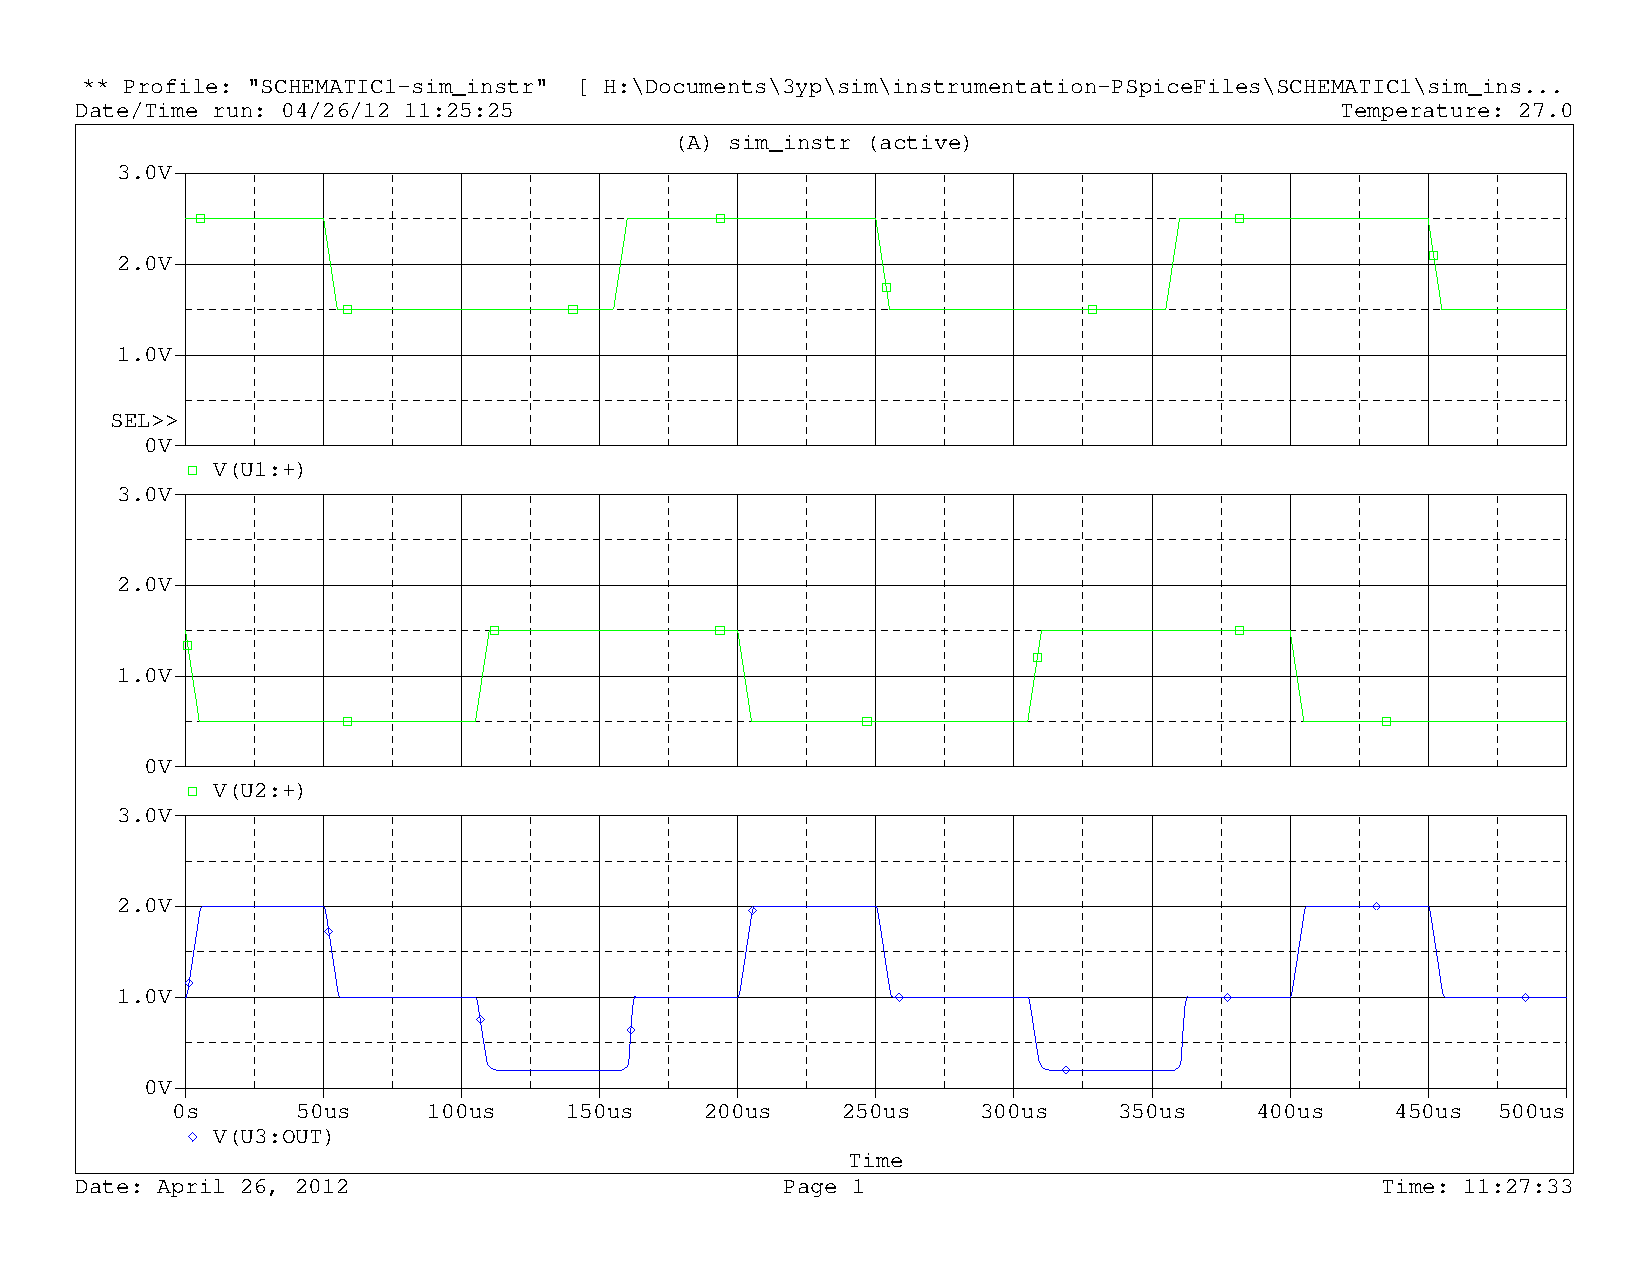
\includegraphics[width=\textwidth]{./img/instrumentationamp_dig.pdf}
	\caption{The output from the instrumentation amplifier from two digital signals}
	\label{fig:instrampbeat}
\end{figure}


\chapter{Implementation}

\chapter{Testing}

\chapter{Evaluation}

\chapter{Conclusions}

\bibliographystyle{plain}
\bibliography{sources}

\appendix
\chapter{PCB Costings}
The costings of the components for the PCB.
The total cost came to \pounds196.90

\begin{table}[H]
	\centering
	\begin{tabular}[c]{| l | l | l | p{50px} | l | l | l |}
		\hline
		\multicolumn{7}{|l|}{MicroControllers} \\
		\hline
		Item	& Component Name& Supplier & Part	& No.	& Unit  & Line \\
		\hline
		DSP	& tms320c6713bpyp200	& Farnell	& 1214441	& 1	& \pounds24.51	& \pounds29.42	\\
		Codec	& wm8988		& Farnell	& 1776294	& 2	& \pounds2.84	& \pounds6.82	\\
		Clock Gen.	& bu2796	& Farnell	& 1716138	& 2	& \pounds0.83	& \pounds1.99	\\
		Dual Op-Amp	& ap358sg	& Farnell	& 1825347	& 10	& \pounds0.08	& \pounds0.96	\\
		\hline
		\multicolumn{7}{|l|}{}\\
		\hline
		\multicolumn{7}{|l|}{Resistors} \\
		\hline
		Item	& Component Name& Supplier & Part	& No.	& Unit  & Line \\
		\hline
		10K\textohm	& r-10k	& Farnell	& 1469748	& 50	& \pounds0.013	& \pounds0.78	\\
		8K2\textohm	& r-8k2	& Farnell	& 9334904	& 50	& \pounds0.01	& \pounds0.60	\\
		1K\textohm	& r-1k	& Farnell	& 9332383	& 50	& \pounds0.025	& \pounds1.50	\\
		120\textohm	& r-120	& Farnell	& 9337059	& 50	& \pounds0.011	& \pounds0.66	\\
		55\textohm	& r-55	& Farnell	& 1500641	& 50	& \pounds0.015	& \pounds0.90	\\
		33\textohm	& r-33	& Farnell	& 1500704	& 50	& \pounds0.016	& \pounds0.96	\\
		8\textohm	& r-8	& Farnell	& 1577385	& 50	& \pounds0.047	& \pounds2.82	\\
		\hline
		\multicolumn{7}{|l|}{}\\
		\hline
		\multicolumn{7}{|l|}{Capacitors} \\
		\hline
		Item	& Component Name& Supplier & Part	& No.	& Unit  & Line  \\
		\hline
		220uF	& c-220u& Farnell	& 1865004	& 5	& \pounds1.10	& \pounds6.60	\\
		10uF	& c-10u	& Farnell	& 1658212	& 10	& \pounds0.115	& \pounds1.38	\\
		4u7F	& c-4u7	& Farnell	& 1759427	& 100	& \pounds0.018	& \pounds2.16	\\
		1uF	& c-1u	& Farnell	& 1759398	& 100	& \pounds0.006	& \pounds0.72	\\
		100nF	& c-0u1	& Farnell	& 1759123	& 100	& \pounds0.005	& \pounds0.60	\\
		1nF	& c-1n	& Farnell	& 1759088	& 100	& \pounds0.005	& \pounds0.60	\\
		8pF	& c-8p	& Farnell	& 1759051	& 100	& \pounds0.006	& \pounds0.72	\\
		\hline
		\multicolumn{7}{|l|}{}\\
		\hline
		\multicolumn{7}{|l|}{Connectors} \\
		\hline
		Item	& Component Name& Supplier & Part	& No.	& Unit  & Line \\
		\hline
		2 pin	& cn-header2	& Farnell	& 1248140	& 10	& \pounds0.106	& \pounds1.24	\\
		8 pin	& cn-header2x4	& Farnell	& 1759051	& 8	& \pounds0.98	& \pounds9.41	\\
		14 pin	& cn-header2x7-box	& Farnell	& 8395926	& 2	& \pounds0.72	& \pounds1.73	\\
		Jack	& cn-st-jack	& Farnell	& 1217016	& 2	& \pounds1.36	& \pounds3.26	\\
		\hline
		\multicolumn{7}{|l|}{}\\
		\hline
		\multicolumn{7}{|l|}{Miscellaneous} \\
		\hline
		Item	& Component Name& Supplier & Part	& No.	& Unit  & Line \\
		\hline
		3.3V Regulator	& ld1117s33	& Farnell	& 1467779	& 2	& \pounds0.71	& \pounds1.71	\\
		1.2V Regulator	& ld1117s12	& Farnell	& 1467778	& 2	& \pounds1.02	& \pounds2.45	\\
		12MHz Crystal	& xtal-12m	& Farnell	& 1652551	& 2	& \pounds0.32	& \pounds0.77	\\
		Red LED		& led-red-0603	& Farnell	& 1465988	& 10	& \pounds0.23	& \pounds2.76	\\
		PCB		&	 	& PCB-Train	& 		& 2	& \pounds78.16	& \pounds78.16	\\
		JTAG Cable	&		& FTDI		& C232HM-DDHSL-0& 1	& \pounds18.50	& \pounds22.20	\\
		Headphones	&		& Play.com	& 3432806	& 1	& \pounds12.99	& \pounds12.99	\\
		\hline
	\end{tabular}
	\caption{Costs involved in the PCB production. Prices correct at time of purchase, line cost includes VAT, unit cost may not}
	\label{tab:pcbcostings}
\end{table}

\chapter{ICA}
Independent Component Analysis (ICA) is a method for separating different signals from a mix.

\section{Methodology}

\section{Limitations}
ICA has some limitations which must be met.
Some of these limitations would result in this algorithm being unsuitable for this project, though these limitations could potentially be circumvented through knowing the circumstances of use.

Under normal circumstances ICA requires at least as many sensors as signal sources.
Without this there isn't enough statistical variation for the different signals to be separated out.
This project only allows for two inputs, one in each ear, which would result in the use of ICA only working for 2 sound sources in the room, which is unlikely to occur, making the use of ICA pointless.
In order to solve this problem certain information about the location and construction of the headphones can be utilised.
The headphones are positioned inside the ear with the microphones pointing outwards.
The ear is shaped in order to direct sound inside the ear, also the microphones are rather directional resulting in 

\section{Implementation}
In the final project ICA was not implemented.
This was largely due to the unexpected length of time taken in implementing the noise cancellation algorithm.


\end{document}
